\section{Luvun desimaaliesitys}

\emph{Desimaaliluvut} on \emph{kymmenjärjestelmään} perustava tapa lukuja.

$123,456$ on esimerkki desimaaliluvusta. Pilkun jälkeen tulevat numerot tarkoittaavat kymmenesosia, sadasosia ja niin edelleen.

\begin{alakohdat}
	\alakohta{$123$ on sen \emph{kokonaisosa}.}
	\alakohta{Kokonaisluku erotetaan loppuosasta \emph{desimaalierottimella}, joka on suomen kielessä pilkku (,).}
	\footnote{Useissa englanninkielisissä maissa käytetään desimaalierottimena pistettä (.) ja pilkku on tuhaterotin. Esimerkiksi yhdysvaltalaisessa kirjassa merkintä \$ 1,000.50 tarkoittaa tuhatta dollaria ja 50 senttiä. Suomen kielessä tuhaterotin on välilyönti.}
	\alakohta{Osaa $456$ kutsutaan luvun \emph{desimaaliosaksi}.}
\end{alakohdat}

\laatikko{

Esimerkkinä annettu desimaaliluku tulkitaan seuraavasti:
\begin{equation*}
123,456 = 1 \cdot 10^2 + 2 \cdot 10^1 + 3 \cdot 10^0 + 4 \cdot 10^{-1} + 5 \cdot 10^{-2} + 6 \cdot 10^{-3}
\end{equation*}

\begin{center}
 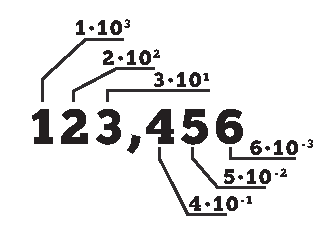
\includegraphics{pictures/Kuva5-1-desimaali-potenssit.pdf}
\end{center}
}

%Kymmenjärjestelmä saa nimensä siitä, että jokainen luvussa esiintyvä %numero kertoo sen paikkaa vastaavien kymmenen potenssien määrän.

\subsubsection*{Murtoluvun muuttaminen desimaaliluvuksi}

Murtoluku on tapa merkitä jakolaskua. Jakolaskun tuloksen esittämiseksi desimaalilukuna
käytetään peruskoulun alaluokilla opetettavaa jakokulmaa. Jakokulman ajatus on yksinkertaisesti kokeilla, kuinka monta jakajaa, sen kymmenesosaa, sadasosaa ja niin
edelleen jaettavaan mahtuu. Jakokulmat voi laskea käsin, laskin tekee saman nopeammin.

\begin{esimerkki}
Muutetaan $\frac{21}{4}$ desimaaliluvuksi laskemalla jakolasku $21 : 4$ jakokulmassa.

\[ 
\begin{array}{cccccc}
 & \underline{ \ \ } & \underline{5}, & \underline{2} & \underline{5} \\
 4 & \!\!|\,2 & 1, & 0 & 0 \\
 \underline{-} & \underline{2}& \underline{0} \\
 & & 1 &0 \\
 & \underline{-} &\underline{ \ \ }  & \underline{8} \\
 & & & 2 & 0 \\
 & & \underline{-} & \underline{2} & \underline{0} \\
 & &  & & 0
\end{array}
\]
Siis $\dfrac{21}{4} = 5,25$.
\end{esimerkki}

Vastaavasti laskien saadaan $\dfrac{3}{11}=0,272727\ldots \ $ :
\[ 
\begin{array}{cccccc}
 & \underline{ 0}, & \underline{2} & \underline{7} & \underline{2} & 
 \underline{\ldots} \\
 11 & \!\!|\,3, & 0 & 0 & 0 & \ldots \\
 \underline{-} & \underline{2}& \underline{2} \\
 & & \boldsymbol{8} &0 \\
 & \underline{-} &\underline{ 7 }  & \underline{7} \\
 & & & \boldsymbol{3} & 0 \\
 & & \underline{-} & \underline{2} & \underline{2} \\
 & &  & & \boldsymbol{8} & 0 \\
 & & & & & \ddots
\end{array}
\]
Koska jakojäännökset 3 ja 8 toistuvat loputtomiin, tämä desimaaliluku
ei ole päättyvä. Siinä on \emph{jakso}: numerosarja 27 toistuu.
Jaksoa voidaan merkitä yläviivan avulla seuraavasti:
\[ 0,27272727\ldots = 0,\overline{27}. \]

{\bf Kaikkien murtolukujen desimaaliesitykset ovat joko päättyviä tai jaksollisia.}
Vähennyslaskuissa syntyvät jakojäännökset ovat nimittäin aina jakajaa pienempiä, ja siksi
ne alkavat väistämättä toistaa itseään, ellei jako jossakin vaiheessa mene tasan.
Koska eri vaihtoehtoja jakojäännöksiksi on yksi jakajaa vähemmän,
jakson pituus on suurimmillaan yhden verran jakajaa pienempi. Esimerkiksi luvulla
$\dfrac{1}{7}=0,\overline{142857}$ jakso on pisin mahdollinen, $7-1=6$ numeron mittainen.

\laatikko{
Tässä on joitain murtolukujen desimaaliesityksiä, jotka on hyvä osata
\begin{alakohdat}
	\alakohta{$ \frac{1}{10} = 0,1$}
	\alakohta{$ \frac{1}{100} = 0,01$}
	\alakohta{$ \frac{1}{2} = 0,5$}
	\alakohta{$ \frac{1}{4} = 0,25$}
	\alakohta{$ \frac{3}{4} = 0,75$}
\end{alakohdat}
}

\subsubsection*{Desimaaliluvun muuttaminen murtoluvuksi}

\paragraph*{Päättyvät desimaaliluvut}

Päättyvät desimaaliluvut voidaan muuttaa murtoluvuiksi muuttamalla kukin
desimaali erikseen murtoluvuksi ja laskemalla syntyneet luvut yhteen.

\begin{esimerkki}
$21,37 = 21+ \frac{3}{10}+\frac{7}{100} =
\frac{2100}{100}+\frac{30}{100}+\frac{7}{100}
 = \frac{2100+30+7}{100} = \frac{2137}{100}.$
\end{esimerkki}

Tämä on turhan työlästä, ja paljon helpommalla päästäänkin kun lavennetaan luku ''niin monella kympillä, kuin siinä on numeroita desimaalipilkun jälkeen''. Täsmällisemmin sanottuna luvulla $10^n$, jossa $n$ on pilkun jälkeen tulevien numeroiden määrä.

\begin{esimerkki}
$21,47 = 21,37 \cdot  \frac{100}{100} = \frac{21,37 \cdot 100}{100} = \frac{2137}{100}$
\end{esimerkki}

%\begin{esimerkki}
%$0,007 = 0,007 \cdot 1 = 0,007 \cdot \frac{10^3}{10^3} = \frac{0,007 \cdot 1000}{1000} = %\frac{7}{1000}$
%\end{esimerkki}

%Menetelmän toimivuus kaikkien desimaalilukujen tapauksessa voidaan todistaa %tarkastelemalla desimaaliluvun määritelmää, mutta jätetään tässä tekemättä.

\paragraph*{Jaksolliset desimaaliluvut}

Minkä tahansa jaksollisen desimaaliluvun voi muuttaa murtoluvuksi seuraavalla tempulla.
Muutetaan esimerkiksi $0,575757\ldots$ murtoluvuksi. Jos merkitään
\[
\begin{array}{rcll}
x &=& \ \, 0,575757 \ldots\ , &\textrm{saadaan sadalla kertomalla} \\
100x &=& 57,575757 \ldots \ , &\textrm{joiden erotuksena} \\
100x - x &=& 57,57 \ldots - 0,57 \ldots \ , & \textrm{eli} \\
99x &=& 57, & \textrm{josta saadaan} \\
x &=& \frac{57}{99} = \frac{19}{33}.
\end{array}
\]
Siis $0,575757\ldots = \frac{19}{33}$. Menetelmä toimii kaikille jaksollisille
desimaaliluvuille: kerrotaan vain sopivalla luvun 10 potenssilla, jotta jakso
katoaa vähennyslaskussa.

\laatikko{
Nämä kannattaa muistaa:
\begin{alakohdat}
	\alakohta{$ \frac{1}{3} = 0,3333 \ldots$}
	\alakohta{$ \frac{2}{3} = 0,6666 \ldots$}
\end{alakohdat}
}

\begin{tehtavasivu}

\begin{tehtava}
Laske ja totea murtolukujen 
 $ \frac{1}{10} = 0,1$ , 
$ \frac{1}{100} = 0,01$ , 
 $ \frac{1}{2} = 0,5$ , 
$ \frac{1}{4} = 0,25$ , 
$ \frac{3}{4} = 0,75$
desimaaliesitysten paikkansapitävyys.
\end{tehtava}

\begin{tehtava}
Muuta murtoluvuksi.
%selkeys voitti täsmällisyyden ei siis murtolukumuotoon
	\begin{alakohdat}
		\alakohta{$43{,}532$}
		\alakohta{$5{,}031$}
		\alakohta{$0{,}23$}
		\alakohta{$0{,}3002$}
		\alakohta{$0{,}101$}
	\end{alakohdat}
\begin{vastaus}
	\begin{alakohdat}
		\alakohta{$ \frac{43532}{1000}$}
		\alakohta{$ \frac{5031}{1000}$}
		\alakohta{$ \frac{23}{100}$}
		\alakohta{$ \frac{3002}{1000}$}
		\alakohta{$ \frac{101}{1000}$}
	\end{alakohdat}
\end{vastaus}
\end{tehtava}

\begin{tehtava}%sovteht tai vaikea tehtävä? sivevennyksen takia
Muuta murtoluvuksi ja sievennä.
%selkeys voitti täsmällisyyden ei siis murtolukumuotoon
	\begin{alakohdat}
		\alakohta{$0{,}01$}
		\alakohta{$0{,}0245$}
		\alakohta{$0{,}004$}
		\alakohta{$0{,}001004$}
	\end{alakohdat}
\begin{vastaus}
	\begin{alakohdat}
		\alakohta{$ \frac{1}{100}$}
		\alakohta{$ \frac{49}{200}$}
		\alakohta{$ \frac{1}{250}$}
		\alakohta{$ \frac{251}{250~000}$}
	\end{alakohdat}
\end{vastaus}
\end{tehtava}

\begin{tehtava}
Muuta murtoluvuksi.
	\begin{alakohdat}
		\alakohta{$0,77777\ldots$}
		\alakohta{$0,151515 \ldots$}
		\alakohta{$2,05\overline{631}$}
		\alakohta{$0,99999\ldots$}
	\end{alakohdat}
\begin{vastaus}
	\begin{alakohdat}
		\alakohta{$\frac{7}{9}$ }
		\alakohta{$\frac{15}{99}=\frac{5}{33}$}
		\alakohta{$\frac{205\ 426}{99\ 900} = \frac{102\ 713}{49\ 950}$}
		\alakohta{$\frac{9}{9} = 1$}
	\end{alakohdat}
\end{vastaus}
\end{tehtava}

\begin{tehtava}
Muuta desimaaliluvuksi.
	\begin{alakohdat}
		\alakohta{$\frac{151}{250}$}
		\alakohta{$\frac{251}{625}$}
		\alakohta{$\frac{386}{1\ 250}$}
		\alakohta{$\frac{493}{500}$}
	\end{alakohdat}
\begin{vastaus}
	\begin{alakohdat}
		\alakohta{$0,604$}
		\alakohta{$0,4016$}
		\alakohta{$0,3088$}
		\alakohta{$0,986$}
	\end{alakohdat}
\end{vastaus}
\end{tehtava}

\begin{tehtava}
Muuta desimaaliluvuksi.
	\begin{alakohdat}
		\alakohta{$\frac{42}{11}$}
		\alakohta{$\frac{37}{13}$}
		\alakohta{$\frac{38}{99}$}
		\alakohta{$\frac{14}{15}$}
	\end{alakohdat}
\begin{vastaus}
	\begin{alakohdat}
		\alakohta{$3,\overline{81}$}
		\alakohta{$2,\overline{846153}$}
		\alakohta{$0,\overline{38}$}
		\alakohta{$0,9\overline{3}$}
	\end{alakohdat}
\end{vastaus}
\end{tehtava}

\begin{tehtava}
	Tunnissa on 60 sekuntia ja minuutissa on 60 sekuntia. Muuta seuraavat ajat tunneiksi.
	\begin{alakohdat}
		\alakohta{73 minuuttia}
		\alakohta{649 sekuntia}
		\alakohta{15 minuuttia ja 50 sekuntia}
		\alakohta{42 minuuttia ja 54 sekuntia}
	\end{alakohdat}
	\begin{vastaus}
		\begin{alakohdat}
			\alakohta{1,21666... tuntia}
			\alakohta{0,1802777... tuntia}
			\alakohta{0,263888... tuntia}
			\alakohta{0,715 tuntia}
		\end{alakohdat}
	\end{vastaus}
\end{tehtava}

\end{tehtavasivu}

\laatikko{
Joissain yhteyksissä käytetään muitakin \emph{lukujärjestelmiä} kuin kymmenjärjestelmää. Esimerkiksi tietokoneet käyttävät kaksikantajärjestelmää eli \emph{binäärijärjestelmää}. Binäärijärjestelmässä jokainen luvun numero kertoo sen paikkaa vastaavan kakkosen potenssien määrän kymmenen potenssien sijasta.

Binäärijärjestelmässä esitetty luku merkitään yleensä kirjoittamalla pieni kakkonen luvun jälkeen, esim. $10,01_2$.
}

\begin{esimerkki}
$10,01_2 = 1 \cdot 2^1 + 0 \cdot 2^0 + 0 \cdot 2^{-1} + 1 \cdot 2^{-2} = 2,25_{10}$
\end{esimerkki}

\begin{tehtavasivu}

\begin{tehtava}
Muunna seuraavat binääriluvut kymmenjärjestelmään.
	\begin{alakohdat}
		\alakohta{$101,0_2$}
		\alakohta{$1,00101_2$}
		\alakohta{$100101,1101_2$}
	\end{alakohdat}
\begin{vastaus}
	\begin{alakohdat}
		\alakohta{$5,0_{10}$}
		\alakohta{$1,15625_{10}$}
		\alakohta{$37.8125_{10}$}
	\end{alakohdat}
\end{vastaus}
\end{tehtava}

\begin{tehtava}
Muunna seuraavat luvut binäärijärjestelmään.
	\begin{alakohdat}
		\alakohta{$7,0_{10}$}
		\alakohta{$2,5_{10}$}
		\alakohta{$11,1875_{10}$}
	\end{alakohdat}
\begin{vastaus}
	\begin{alakohdat}
		\alakohta{$111,0_2$}
		\alakohta{$10,1_2$}
		\alakohta{$1011,0011_2$}
	\end{alakohdat}
\end{vastaus}
\end{tehtava}

\end{tehtavasivu}
